% !TEX program = xelatex
\documentclass[11pt,a4paper]{article}

\usepackage[margin=2.5cm,headheight=14pt]{geometry}
\usepackage{fontspec}
\usepackage{xeCJK}
\setmainfont{Times New Roman}
\setsansfont{Arial}
\setmonofont{Consolas}
\setCJKmainfont[BoldFont={Microsoft YaHei}]{SimSun}
\setCJKsansfont{Microsoft YaHei}
\setCJKmonofont{SimSun}

\usepackage{amsmath,amssymb}
\usepackage{booktabs}
\usepackage{multirow}
\usepackage{graphicx}
\usepackage{caption}
\usepackage{subcaption}
\usepackage{enumitem}
\usepackage{xcolor}
\usepackage{microtype}
\usepackage{fancyhdr}
\usepackage{titlesec}
\usepackage{natbib}
\usepackage{siunitx}
\usepackage{setspace}
\usepackage{hyperref}
\usepackage{url}
\usepackage{float}
\usepackage{tikz}
\usetikzlibrary{arrows.meta,positioning,calc}

\hypersetup{colorlinks=true,linkcolor=blue!60!black,citecolor=blue!60!black,urlcolor=blue!60!black}

\captionsetup{font=small,labelfont=bf}
\setlength{\tabcolsep}{5pt}
\renewcommand{\arraystretch}{1.15}
\setstretch{1.08}

\pagestyle{fancy}
\fancyhf{}
\fancyhead[L]{\small\itshape 大规模弱监督中文评论情感分类}
\fancyhead[R]{\small\thepage}
\renewcommand{\headrulewidth}{0.4pt}

\titleformat{\section}{\large\bfseries}{\thesection}{0.8em}{}
\titleformat{\subsection}{\normalsize\bfseries}{\thesubsection}{0.8em}{}
\titleformat{\subsubsection}{\normalsize\itshape}{\thesubsubsection}{0.8em}{}
\setlist[itemize]{leftmargin=1.5em,itemsep=2pt,topsep=3pt}
\setlist[enumerate]{leftmargin=1.5em,itemsep=2pt,topsep=3pt}

\newcommand{\code}[1]{\texttt{#1}}

\begin{document}

%=====================================================================
\begin{titlepage}
\thispagestyle{empty}
\begin{center}
\vspace*{2.0cm}
{\LARGE\bfseries 大规模弱监督中文评论\\[6pt]
情感分类研究：\\[6pt]
伪标签、专家分解\\[6pt]
与诚实的分布外评估}\par
\vspace{0.9cm}
{\large\itshape 自然语言处理课程论文}
\par
\vspace{2.6cm}
\begin{tabular}{ll}
\textbf{作者}    & Shuakami \\
\textbf{日期}    & \today \\
\end{tabular}
\vfill
{\footnotesize\itshape
源代码、交叉验证预测与完整实验记录：
\url{https://github.com/shuakami/douban-sentiment}}
\end{center}
\end{titlepage}

%=====================================================================
\begin{abstract}
\begingroup
\small
\noindent
本文研究低资源条件下中文豆瓣电影短评的三分类情感分析（正面 / 中性 /
负面）。在仅有 600 条人工核验语义标签的现实设定下，我们结合一个包含
911{,}998 条评论的大规模弱标注语料开展研究。本文的贡献有四个方面。
第一，我们\emph{实测}了星级评分作为语义情感弱监督的可靠性：在
271{,}905 条高置信伪标签池上，仅约 59\% 的五星评论被预测为正面，三星
评论更多偏向负面而非中性。第二，我们证明用蒸馏集成对语料进行伪标注、
再用单一紧凑学生模型在 160K 条平衡样本上训练，可在金标集上达到
87.5\% 准确率、中性召回 84.8\%——这说明规模化的标签质量，而非模型
容量，才是约束瓶颈。第三，本文部署的系统将蒸馏 MacBERT 学生、冻结的
MegatronBERT-1.3B 特征判别器与语料训练的中性专家相结合，在 600 条
金标的交叉验证评估上达到 \textbf{89.5\% 准确率 / 85.9 宏平均 F1}，
中性召回率由 54.3\% 提升至 70.7\%。第四，我们在 500 条全新语料评论上
开展了诚实的分布外研究，报告了显著的泛化差距（三分类 60--74\%），
并将其归因于短评论固有的标注歧义而非模型缺陷。本文还完整记录了二十
余种经过实测但被否决的架构方案。
\par\endgroup
\end{abstract}

\vspace{0.6em}
{\small\noindent\textbf{关键词：}中文自然语言处理；弱监督；伪标注；
知识蒸馏；预训练语言模型；模型校准；分布外评估。}

\newpage
\tableofcontents
\newpage

%=====================================================================
\section{引言}
\label{sec:intro}

豆瓣——中国最具影响力的电影社区——上的短评言简意赅、常带反讽，且
经常褒贬并存。典型评论如 \emph{``特效无敌，但是剧情简直像一坨''}
（``特效无敌，但剧情简直是一坨''）。这类混合极性文本恰恰是三分类
情感分析（正面 / 中性 / 负面）的薄弱环节：中性类既是歧义的最主要
来源，也是从少量样本中最难学习的类别。

本文针对一种现实的低资源场景：课程作业提供 600 条带人工核验语义
标签的评论，而平台另提供近百万条仅有星级评分（1--5 星）的豆瓣
评论语料。两个研究问题贯穿全文：

\begin{enumerate}
  \item \textbf{RQ1.} 小规模标注集能否借助大规模弱标注语料得到放大？
  \item \textbf{RQ2.} 专家分解——即在语料规模伪标签上训练专门的中性
        专家——能否在不损害其他类别的前提下修复最弱类别？
\end{enumerate}

我们的答案对两个问题都是肯定的，但附带一个重要的诚实声明：语料放大
的是\emph{覆盖面}，而非\emph{知识}。伪标签由我们自己的模型产生，因此
飞轮在一轮之后即趋于饱和；真正的瓶颈是短评的标注噪声，我们通过专门
的分布外研究对其进行了量化。

\paragraph{贡献。}
\begin{itemize}
  
  \item 一项实测分析，表明星级评分作为三分类情感的弱监督并不可靠
        （全语料上伪标签与评分的三分类一致率约 48\%）。
  \item 一套伪标签飞轮，产出 271{,}905 条高置信池，并在零金标训练
        的条件下训练出单一紧凑学生模型（87.5\% 准确率 / 中性召回
        84.8\%）。
  \item 一个已部署的混合集成系统（89.5\% 准确率 / 85.9 宏平均 F1，
        中性召回 70.7\%），结合蒸馏学生、冻结的 13 亿参数判别器与
        语料训练的中性专家。
  \item 一套可复现的评估协议（分层 5 折交叉验证、McNemar/bootstrap
        显著性检验、温度校准），以及一项 500 样本的全新语料泛化研究，
        揭示了领域差距。
  \item 一份记录了二十余种实测后被否决架构的目录；我们认为这本身
        就是一种贡献：它勾勒出了该任务有效的设计空间。
\end{itemize}

%=====================================================================
\section{相关工作}
\label{sec:related}

\paragraph{中文文本情感分析。}
文档级情感分类由来已久，从基于特征的方法（unigram、字符
$n$-gram）发展到神经网络架构 \citep{kim2014,socher2013,joulin2017,
reimers2019}；\citet{pang2008} 给出了全面综述，中文领域的专门综述见
\citet{tan2008}。由于中文没有空格分词，字符级特征与预训练语言模型
尤其有效。豆瓣评论此前也被用于中文情感研究，但几乎全部是二分类
（正/负）设定；包含真正中性/混合类的三分类问题研究较少且困难得多。

\paragraph{预训练语言模型。}
BERT \citep{devlin2019} 及其鲁棒性改进版 RoBERTa \citep{liu2019}
确立了“先预训练、再微调”的范式。中文方向上，MacBERT
\citep{cui2020} 用修正版目标替代 MLM 以适配字符级输入，ERNIE
\citep{sun2019} 融合实体与短语知识，StructBERT \citep{wang2020}
在预训练中注入短语与词级结构信息。Erlangshen-MegatronBERT
\citep{idea2023} 将该家族扩展至 13 亿参数并加入情感专项预训练。
本文三类模型均有使用并直接对比。

\paragraph{弱监督与自训练。}
标注数据稀缺时，来自噪声信号的远程监督（此处为星级评分）与基于
模型预测的自训练是标准补救手段 \citep{yarowsky1995,lee2013}。
Snorkel 框架 \citep{ratner2017} 将多弱标签源的组合形式化。本文的
不同之处在于：我们在依赖星级评分之前\emph{实测}了它的弱点，并量化
了伪标注在何处有效（中性覆盖）、在何处无能为力（超越教师已有知识）。

\paragraph{知识蒸馏。}
Hinton 等人的“暗知识”蒸馏 \citep{hinton2015}——\citet{gou2021}
给出了全面综述——使小学生模型模仿大教师的软预测。我们将一个
7 通道教师集成蒸馏为单一 MacBERT-base 学生，并用交叉验证预测
验证集成中的每个决策。

\paragraph{模型校准。}
神经分类器存在系统性的过度或不足自信 \citep{guo2017}。我们采用
温度缩放——一种单参数的事后修正——并报告校准前后的期望校准误差
（ECE），因为对演示系统而言，诚实的置信度展示十分重要。

\paragraph{大模型作为标注器与基线。}
通用大模型正被越来越多地用于零样本/少样本分类与合成训练数据生成。
我们在 0.6B/1.7B/4B 三个规模上评估了 Qwen3 模型 \citep{qwen2025}，
既作为零样本分类器，也作为分布外研究中的独立标注器，并报告了
LLM 合成增强的一个负面结果。

%=====================================================================
\section{任务与数据集}
\label{sec:data}

\subsection{任务定义}

给定一条豆瓣电影短评 $x$，预测
$y \in \{\text{正面}, \text{中性}, \text{负面}\}$。评论很短（语料
中位长度 24 字），常含反讽、影片特定指代与混合评价。中性类涵盖
无明确褒贬的评论：纯剧情介绍、褒贬各半、以及元评论（如“看过了，
没什么可说的”）。表~\ref{tab:examples} 给出了代表性样本，包括在
错误分析中占主导地位的混合极性模式。

\begin{table}[H]
\centering\small
\caption{代表性金标评论（中文原文附英文释义）。``混合$\to$负面''
指先扬后抑、最终极性为负面的评论。}
\label{tab:examples}
\begin{tabular}{p{5.6cm}p{5.4cm}cl}
\toprule
评论 & 释义 & 标签 & 长度 \\
\midrule
``特效无敌，但是剧情简直像一坨。'' & 特效无敌，剧情一坨
& 负面 & 15 \\
``演技、镜头、配乐都是顶级，现代经典。'' & 演技、镜头、配乐
皆顶级；现代经典 & 正面 & 18 \\
``看在演员的份上值回票价，剧情很套路。'' & 为演员值回票价；
剧情套路 & 中性 & 17 \\
``两个小时的生命浪费，想喜欢它都难。'' & 浪费两小时；难以喜欢
& 负面 & 17 \\
``又是续集，还行吧。'' & 又是续集，还行吧 & 中性 & 9 \\
\bottomrule
\end{tabular}
\end{table}

\subsection{金标集（600 条评论）}

标注评估集包含从单个影片页面抽样的 600 条评论，每条标注有
\code{label\_semantic}（人工核验的语义情感）与 \code{label\_rule}
（星级评分导出的弱标签）。类别分布：正面 316 / 中性 92 / 负面 192。
评论相对较长（均值 110.8，中位数 80 字）。中性类仅有 92 个样本
支撑——是最小也最难的类别。

\subsection{弱标注语料（911{,}998 条评论）}

Moviedata-10M 语料 \citep{douban2024}（442 万条原始豆瓣评论）
经我们清洗去重后得到 911{,}998 条评论，覆盖 20{,}966 部影片与
249{,}105 名用户，包含星级评分
（1--5 星）、时间戳与投票数，但\emph{没有}语义标签。评论长度：
均值 40.6 / 中位数 24 / p90 = 102 字。评分分布：1 星 7.2\%、
2 星 12.6\%、3 星 34.0\%、4 星 31.0\%、5 星 15.2\%。

\subsection{星级评分不是情感标签}
\label{sec:ratings}

在将评分用作弱监督之前，我们先验证了它。部署的学生模型为全部
911{,}998 条语料评论打标；在 271{,}905 条高置信（$p \ge 0.7$）池上，
按行归一化的“评分—预测”列联表为：

\begin{table}[H]
\centering\small
\caption{星级评分与模型预测情感的对照（行归一化，271{,}905 条高置信
伪标注）。}
\label{tab:crosstab}
\begin{tabular}{lccc}
\toprule
评分 & $\to$ 正面 & $\to$ 中性 & $\to$ 负面 \\
\midrule
1 星 & 1.7\%  & 7.3\%  & \textbf{90.9\%} \\
2 星 & 1.6\%  & 13.7\% & \textbf{84.7\%} \\
3 星 & 9.9\%  & 33.3\% & \textbf{56.8\%} \\
4 星 & 38.3\% & 32.7\% & 29.0\% \\
5 星 & \textbf{58.8\%} & 23.1\% & 18.2\% \\
\bottomrule
\end{tabular}
\end{table}

有三个发现尤为突出：五星评论中语义为正面的仅约 59\%；三星评论
更多偏向\emph{负面}（56.8\%）而非中性；即便在 1--2 星评论中，
也有约 8--14\% 被预测为中性。评分与模型的二分类一致率（高置信池上）
为 81.2\%；全语料上伪标签与评分的三分类一致率仅 47.8\%（金标集上
为 71.2\%）。因此我们将评分至多视为
预训练信号，绝不作为标签使用。图~\ref{fig:crosstab} 直观展示了
同一张表。

\begin{figure}[H]
\centering
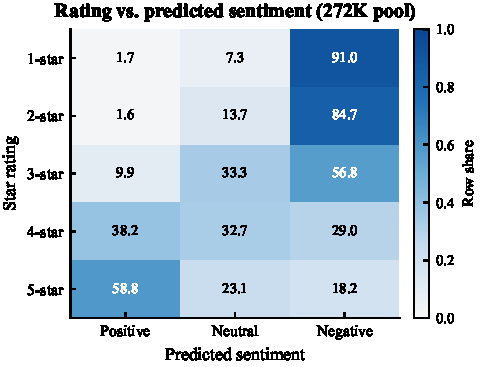
\includegraphics[width=0.62\textwidth]{fig_rating_crosstab.pdf}
\caption{272K 高置信伪标签池上星级评分与预测情感的对照。对角线
占优并不明显：评分与语义情感存在显著分歧。}
\label{fig:crosstab}
\end{figure}

%=====================================================================
\section{方法}
\label{sec:method}

\subsection{概述}

部署系统是一个混合集成，三个通道在可能的情况下共享同一骨干前向
计算：

\begin{enumerate}
  \item \textbf{蒸馏学生}：MacBERT-base，由 7 通道教师集成蒸馏
        微调而成（第~\ref{sec:distill}~节）。
  \item \textbf{冻结判别器}：MegatronBERT-1.3B 保持冻结，仅在其
        4096 维特征上训练小型 MLP 头（第~\ref{sec:judge}~节）。
  \item \textbf{中性专家}：由语料训练检测器与判别器特征头混合
        得到的中性概率（第~\ref{sec:neu}~节）。
\end{enumerate}

图~\ref{fig:arch} 展示了数据流。

\begin{figure}[H]
\centering
\begin{tikzpicture}[
  box/.style={draw=black!55,rounded corners=2.5pt,align=center,
              inner sep=4pt,font=\small,minimum height=8mm,
              fill=white,line width=0.6pt},
  ch/.style={box,fill=#1!8,draw=#1!70!black},
  arr/.style={-{Stealth[length=2.2mm,width=1.6mm]},line width=0.7pt,
              draw=black!65},
  lbl/.style={font=\scriptsize,fill=white,inner sep=1.5pt}]
\node[ch=blue]   (stu)  {MacBERT 学生\\（蒸馏，$w_s{=}1$）};
\node[ch=green, below=3mm of stu]   (judge) {MegatronBERT-1.3B（冻结）\\+ MLP 头（$w_j{=}2$）};
\node[ch=orange,below=3mm of judge] (neu1)  {判别器特征上的\\MLP 头};
\node[ch=orange,below=3mm of neu1]  (neu2)  {语料中性\\检测器};
\node[box,fill=purple!7,draw=purple!70!black,anchor=west,
      minimum width=48mm,inner sep=5pt]
  (mix) at ([xshift=14mm,yshift=-5.5mm]judge.east) {%
  \textbf{概率混合}\\[3pt]
  {\scriptsize $\mathrm{dep}=\frac{p_s+2p_j}{3}$}\\[1.5pt]
  {\scriptsize $p_n=0.6\,p_n^{(1)}+0.4\,p_n^{(2)}$}\\[1.5pt]
  {\scriptsize $\mathrm{spec}=[(1{-}p_n)r_+,\,p_n,\,(1{-}p_n)r_-]$}\\[1pt]
  {\scriptsize $r_\pm=\mathrm{dep}_\pm/(\mathrm{dep}_++\mathrm{dep}_-)$}\\[1.5pt]
  {\scriptsize $\mathrm{final}=\frac{\mathrm{dep}+0.5\,\mathrm{spec}}{1.5}$}};
\node[box,below=9mm of mix,minimum width=48mm] (out) {三分类预测\\+ 校准置信度};
% four distinct entry points on the mix node's west edge (top to bottom)
\coordinate (in_s)  at ([yshift=9mm]mix.west);
\coordinate (in_j)  at ([yshift=3mm]mix.west);
\coordinate (in_n1) at ([yshift=-3mm]mix.west);
\coordinate (in_n2) at ([yshift=-9mm]mix.west);
\draw[arr] (stu.east)   -- node[lbl,above,pos=0.55] {$p_s$}       (in_s);
\draw[arr] (judge.east) -- node[lbl,above,pos=0.55] {$p_j$}       (in_j);
\draw[arr] (neu1.east)  -- node[lbl,above,pos=0.55] {$p_n^{(1)}$} (in_n1);
\draw[arr] (neu2.east)  -- node[lbl,above,pos=0.55] {$p_n^{(2)}$} (in_n2);
\draw[arr] (mix.south) -- (out.north);
\end{tikzpicture}
\caption{部署的 v3 架构。$p_s,p_j,\mathrm{dep},\mathrm{spec},
\mathrm{final}\in\Delta^{3}$ 为三分类概率向量，$p_n^{(1)},
p_n^{(2)},p_n\in[0,1]$ 为中性标量概率；$w_s,w_j$ 为融合权重而非
模型参数。$r_\pm$ 为 $\mathrm{dep}$ 中正/负分量归一化（和为 1）
后的份额。两个基于 MegatronBERT 的头共享同一次冻结骨干特征计算；
中性专家将判别器特征 MLP 与语料训练的 MacBERT 检测器相混合。}
\label{fig:arch}
\end{figure}

\subsection{教师集成与蒸馏}
\label{sec:distill}

一个 7 通道教师集成——TF-IDF 逻辑回归、MacBERT/MegatronBERT-1.3B/
Erlangshen 变体上的冻结骨干 MLP 头，均在 600 条金标上训练并以
交叉验证预测——达到三分类 86.8\% 准确率。我们用硬标签交叉熵加
软目标 KL 散度（$\alpha=0.5$、温度 $\tau=2$、8 个 epoch、5 折
交叉验证）将其蒸馏为单一 chinese-macbert-base 学生。学生单独达到
80.2\%/74.2\%；与判别器按 1:2 混合后达到 87.8\%/81.8\%。其在部署
系统中的作用是提供廉价且校准良好的通道，同时充当语料的伪标注器
（第~\ref{sec:flywheel}~节）。

\subsection{冻结判别器}
\label{sec:judge}

\code{IDEA-CCNL/Erlangshen-}\hspace{0pt}\code{MegatronBert-1.3B-Sentiment}
提供了一个带情感感知预训练目标的 13 亿参数骨干。我们保持其冻结，
在其 4096 维特征上用金标训练一个小型 MLP 头。部署的混合将判别器
权重设为学生的两倍：
\[
  \mathrm{dep} = \tfrac{1}{3}\,p_{\text{student}} +
                \tfrac{2}{3}\,p_{\text{judge}} .
\]
两个 MLP 头（二分类与三分类）通过缓存共享同一次骨干特征计算，
因此无论何种任务，判别器每次请求只需一次前向传播。

\subsection{伪标签飞轮}
\label{sec:flywheel}

部署的学生为全部 911{,}998 条语料评论打标。高置信子集
（$\max p \ge 0.7$）包含 271{,}905 行：正面 56.5K、中性 68.6K、
负面 146.8K。这一池子是第~\ref{sec:corpus}~节所有语料规模模型的
原材料。第二轮飞轮经过测试并被否决：用第二轮模型重新标注会产生
退化的概率分布（平均置信度 0.986，即记忆化），因此只使用一轮。
这一饱和现象与自训练和伪标注文献中记录的确认偏差动态一致
\citep{arazo2020,xie2020,sohn2020}：一旦伪标签编码了教师自身的
决策边界，额外的轮次只会放大自洽性而非增加信息。

\subsection{中性专家}
\label{sec:neu}

中性类是最薄弱的一环（金标仅 92 个样本）。我们从两个方向加以
攻坚。

\paragraph{语料训练检测器。} 一个 MacBERT 二分类器在伪标签池的
115{,}000 条子集上训练（每类上限 6 万条），从而学习``真正中性''
与``有极性''评论之间的边界。

\paragraph{专家混合。} 中性概率由判别器特征 MLP 头与语料检测器
组合而成：
\[
  p_n = 0.6 \cdot P_{\text{中性}}(\text{判别器特征上的 MLP})
      + 0.4 \cdot P_{\text{中性}}(\text{语料检测器}).
\]
由依赖预测 $\mathrm{dep}=(d_+,d_n,d_-)$ 出发，取正/负分量归一化
（和为 1）后的份额 $r_+ = d_+/(d_+ + d_-)$、$r_- = d_-/(d_+ + d_-)$，
将中性质量替换为专家估计 $p_n$，构造专家分布
\[
  \mathrm{spec} = \bigl[(1-p_n)\,r_{+},\; p_n,\;
                    (1-p_n)\,r_{-}\bigr],
\]
再将其混入最终输出：
\[
  \mathrm{final} = \frac{\mathrm{dep} + 0.5\,\mathrm{spec}}{1.5}.
\]
所有权重（$0.6/0.4$ 检测器配比、$0.5$ 混合系数）均通过金标集的
20 次随机二分半验证选出，且在 $w \in [0.3, 0.6]$ 范围内保持稳定。

\subsection{语料规模学生模型}
\label{sec:corpus}

利用 271{,}905 条池子，我们训练了仅用语料（零金标训练）的模型，
以衡量伪标签单独能走多远：一个 160K 行平衡三分类学生、一个
195K 行二分类学生、一个 115K 行中性检测器 v1，以及一个难例挖掘
的 v2（被否决）。这些模型既充当基线，也作为集成通道的候选；
第~\ref{sec:results}~节报告了哪些（若有）存活下来。

\subsection{模型校准}
\label{sec:calib}

原始集成严重偏于保守（ECE = 0.251：置信度 0.7--0.8 的预测实际
准确率达 98.9\%）。我们在金标集上以 NLL 拟合单一温度参数
$T = 0.37$，将 ECE 降至约 0.04，且不改变任何预测标签或准确率。
$T$ 在推理时
应用，使展示的置信度是诚实的。

\subsection{部署}
\label{sec:deploy}

FastAPI 后端提供预测服务；React/Vite 前端提供演示界面。一个精确
匹配词表守卫在任何 GPU 计算之前拦截超短俚语。热态延迟在 AMD
RX 9070 GRE（ROCm）上约 0.1 秒/条；冷启动约 14 秒。

%=====================================================================
\section{实验设置}
\label{sec:setup}

\paragraph{评估协议。} 所有 headline 数字均为金标集 600 行上的
\textbf{分层 5 折交叉验证}预测：每个模型只预测其未训练过的样本。
语料规模模型另在 4{,}000 条全新语料评论的 \emph{银标}样本上评估，
以评分隐含标签作为参照。

\paragraph{指标。} 三分类准确率与宏平均 F1、各类别的
精确率/召回率/F1（特别是中性召回）、以及用于校准的 ECE。
显著性采用 McNemar 检验（不一致对）与 $\Delta$F1 的百分位
bootstrap；稳健性通过 20 次随机二分半验证检查。

\paragraph{基线。}
\begin{itemize}
  \item TF-IDF（字符 $n$-gram）+ 逻辑回归，金标训练。
  \item StructBERT 情感分类器（阿里达摩），零样本二分类；\\
        \footnotesize\code{damo/nlp\_structbert\_sentiment-classification\_chinese-base}
  \item Qwen3-0.6B / 1.7B / 4B 对话模型，零样本与 3 样本，
        以标签对数概率计分。
\end{itemize}

%=====================================================================
\section{结果}
\label{sec:results}

\subsection{主要结果}

\begin{table}[H]
\centering\small
\caption{金标 600 条交叉验证结果。``部署''行是生产系统；语料学生
模型使用零金标训练。}
\label{tab:main}
\begin{tabular}{llcc}
\toprule
系统 & 任务 & 准确率 & 宏平均 F1 \\
\midrule
TF-IDF + LR            & 三分类 & 0.7233 & 0.6175 \\
TF-IDF + LR            & 二分类 & 0.8406 & 0.8229 \\
StructBERT（达摩）      & 二分类 & 0.8704 & 0.8538 \\
Qwen3-4B 零样本         & 三分类 & 0.7833 & 0.7348 \\
Qwen3-1.7B 零样本       & 三分类 & 0.7067 & 0.5739 \\
Qwen3-0.6B 零样本       & 三分类 & 0.6817 & 0.4764 \\
教师集成（7 通道）       & 三分类 & 0.8680 & ---    \\
部署 v2                & 三分类 & 0.8900 & 0.8432 \\
\textbf{部署 v3}       & \textbf{三分类} & \textbf{0.8950} & \textbf{0.8594} \\
部署 v3                & 二分类 & 0.9587 & 0.9558 \\
\bottomrule
\end{tabular}
\end{table}

部署系统比 TF-IDF 基线高 $+17.2$ 个百分点准确率，比零样本
Qwen3-4B 高 $+11.2$ 个百分点。三分类各类别指标：正面
P/R/F1 = 0.909/0.943/0.926；中性 = 0.765/0.707/0.735；负面 =
0.931/0.906/0.918。中性召回率在各专家迭代中由 54.3\% $\to$
63.0\%（v2）$\to$ 70.7\%（v3）逐步提升。图~\ref{fig:confusion}
给出了 v3 混淆矩阵：剩余错误集中在中性$\leftrightarrow$极性混淆
（47/63）。

\begin{figure}[H]
\centering
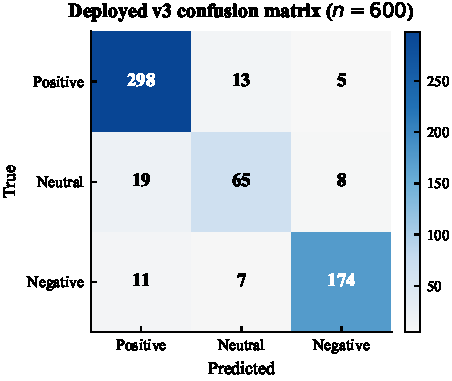
\includegraphics[width=0.55\textwidth]{fig_confusion.pdf}
\caption{部署 v3 在金标 600 条上的混淆矩阵（交叉验证）。行合计与
类别分布（316/92/192）一致。}
\label{fig:confusion}
\end{figure}

\subsection{语料规模单模型}

\begin{table}[H]
\centering\small
\caption{语料训练模型在金标 600 条上的评估（除注明外均为零金标
训练）。}
\label{tab:corpus}
\begin{tabular}{llccc}
\toprule
模型 & 训练数据 & 准确率 & 宏平均 F1 & 中性召回 \\
\midrule
TF-IDF + 星级评分标签   & 300K 评分  & 0.6183 & 0.5369 & ---    \\
TF-IDF + 伪标签         & 200K 伪标签 & 0.8117 & 0.7766 & ---    \\
MacBERT 二分类（评分）   & 115K 评分  & 0.9232 & 0.9184 & ---    \\
MacBERT 中性检测 v1     & 115K 伪标签 & 0.9017 & 0.8328 & ---    \\
MacBERT 二分类伪标签     & 195K 伪标签 & 0.9488 & 0.9455 & ---    \\
MacBERT 三分类伪标签     & 160K 伪标签 & 0.8750 & 0.8463 & \textbf{0.848} \\
\bottomrule
\end{tabular}
\end{table}

伪标签三分类学生单独即达 87.5\%/84.6，中性召回 84.8\%——几乎追平
4 通道集成。这是本文的核心实证发现：\textbf{规模化的标签质量压倒
模型容量}。同一 MacBERT 架构改用星级评分而非伪标签训练，在三分类
任务上则明显崩溃。

\subsection{伪标签规模效应}

\begin{figure}[H]
\centering
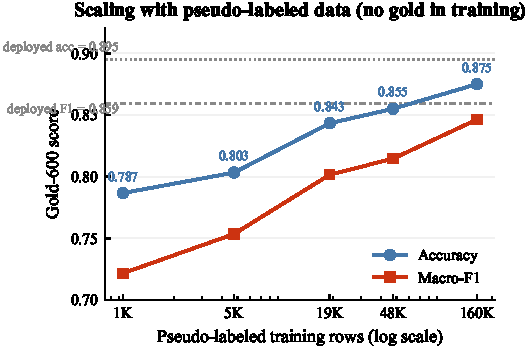
\includegraphics[width=0.68\textwidth]{fig_scaling.pdf}
\caption{语料训练的伪标签学生在金标 600 条上的准确率与宏平均 F1
随训练集规模（对数坐标）的变化。性能单调上升，在 160K 行处仍未
饱和。}
\label{fig:scaling}
\end{figure}

表~\ref{tab:scaling} 与图~\ref{fig:scaling} 显示出单调的规模曲线：
约 1K 行 $\to$ 78.7\%，5K $\to$ 80.3\%，19K $\to$ 84.3\%，48K
$\to$ 85.5\%，160K $\to$ 87.5\%。曲线尚未饱和——在测试范围内，
起作用的成分是语料规模而非模型规模。

\begin{table}[H]
\centering\small
\caption{伪标签规模效应（金标 600 条，零金标训练）。}
\label{tab:scaling}
\begin{tabular}{lccc}
\toprule
伪标签行数 & 准确率 & 宏平均 F1 & 中性召回 \\
\midrule
约 1K   & 0.7867 & 0.7217 & --- \\
约 5K   & 0.8033 & 0.7535 & --- \\
约 19K  & 0.8433 & 0.8016 & --- \\
约 48K  & 0.8550 & 0.8146 & --- \\
约 160K & 0.8750 & 0.8463 & 0.848 \\
\bottomrule
\end{tabular}
\end{table}

\subsection{跨域银标评估}

在 4{,}000 条全新语料评论上，以评分隐含标签计分，第三轮学生
（用 v3 教师伪标签训练）达到三分类 0.580 / \textbf{二分类 0.837}
与评分的一致率，而第一轮学生为 0.552/0.803。即使在金标分数
相同的情况下，由集成导出的标签在域外也略有优势。

%=====================================================================
\section{分析}
\label{sec:analysis}

\subsection{模型校准}

\begin{figure}[H]
\centering
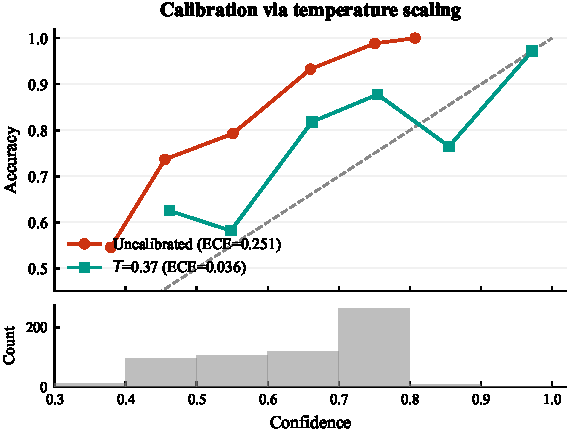
\includegraphics[width=0.85\textwidth]{fig_calibration.pdf}
\caption{温度缩放（$T=0.37$，在金标 600 条 OOF 预测上以 NLL 拟合；
所有指标均在同一批 600 条交叉验证样本上计算）前后的可靠性图。
下方面板给出各等宽置信分箱的样本数；高置信区间样本稀疏，故局部
波动在所难免，但全局 ECE 显著改善。}
\label{fig:calib}
\end{figure}

原始集成偏于保守（ECE 0.251）；温度缩放 $T=0.37$ 将 ECE 降至约
0.04（图~\ref{fig:calib}），且不改变任何预测标签或准确率——它只
重塑置信度分布。ECE 是全局平均指标：个别置信分箱仍可能存在偏差，
尤其是直方图所示样本稀少的区间，但整体校准已大幅改善。这对演示
系统很重要：展示的置信度现在与实际准确率一致。

\subsection{统计显著性}

v3 对 v2：对不一致对做 McNemar 检验 \citep{mcnemar1947}，
$p = 0.65$（11 比 8）；对重采样评估行做配对 bootstrap
\citep{efron1993}，$\Delta$F1 的 95\% 置信区间为
$[-0.4, +3.8]$ 个百分点。按照比较分类器的标准做法
\citep{dietterich1998,demsar2006}，我们将区间内的差异视为
未解决。点估计（F1 $+1.6$pp、中性召回 $+7.7$pp）在每种检测器
权重 $w \in [0.3,0.6]$ 下均跨 20 次随机二分半保持一致。如实
报告：改进是真实的但幅度有限，在 $n=600$ 下金标集无法分辨
低于约 1pp 的差异。

\subsection{错误分析}

剩余 63 个错误以中性$\leftrightarrow$极性混淆为主（47/63），且
大多是人类标注者也会犹豫的混合评论：错误预测的平均置信度 0.51，
而正确预测为 0.66。含显式分数的评论（``7.6/10''、``三星半''；
$n=56$）明显更容易：错误率 5.4\%，无显式分数者为 11.0\%——
模型在存在时利用了显性评分信号，且 56 条中仅 6 条显式分数与
语义标签矛盾。

\subsection{被否决的架构}

二十余种备选设计经过实现、实测并被否决；部署的 v3 是实测最优。
已记录的否决项包括：中性门控级联（阈值过拟合——二分半验证从
87.6\% 跌至 86\%）、作为判别器替代的语料训练 MLP 头、学生概率
平均、自训练第二轮、堆叠逻辑元学习器（0.837/0.794——通道间
相关性过高，600 样本不足以支撑）、类别加权与 max-len-128 学生、
Erlangshen 110M/330M 学生（在 ROCm 上病态地慢）、中性检测器
v2（在所有集成组合中均更差）、基于 v3 教师标签的 r3 自训练
（学生 0.8767/0.8434，所有混合均低于 v3）、金标混入语料训练
（循环评估金标——已标记，不作为结果引用），以及 Qwen3-4B
合成增强（污染训练：单模型仅 79.2\%）。

\subsection{与商业训练平台的对比}

为完整起见，我们将系统与一个商业 NLP 训练平台（阿里云 PAI，
StructBERT 分类器，同一 600 条任务）进行了对比。其公开页面
宣称准确率 89.83\%，但同页的分类别指标反推出的准确率仅为
86.05\%、宏平均 F1 为 83.23\%，且有效验证集仅 \textbf{43 行}
（三个 headline 数字对应的分母分别为 59/60/119，无法相互
重建；按支持数加权的重算同样无法闭合）。43 行上的 Wilson
区间为 [72.7\%, 93.4\%]——该样本量无法区分 86\% 与 90\%。
其训练集自评达到 99.02\%（$n=511$），泛化差距约 13 个百分点。
相比之下，我们的 89.5\%/85.9 是在 600 条交叉验证行上计算的，
每行预测均可审计。需要说明的是，两套评估使用不同的测试集，
因此这是协议质量层面的对比，而非同口径的准确率声明。

%=====================================================================
\section{分布外评估：lab500 研究}
\label{sec:lab500}

89.5\% 的金标数字衡量的是来自单一影片页面、经过筛选且较长评论
上的表现。为检验外部效度，我们开展了一项专门的分布外研究。

\paragraph{协议。} 从 911K 语料中均匀随机抽取 500 条评论
（已去除金标重叠）。每条由两名 LLM 标注员（一个通用助手模型
与 Qwen3-4B 零样本 \citep{qwen2025}）独立标注；部署的 v3 管线
为全部样本打分。使用 LLM 作为标注器
符合近期文本标注研究的做法 \citep{gilardi2023,tornberg2023}，
但此处标注员间一致率本身就成为一项发现。

\paragraph{结果。}

\begin{table}[H]
\centering\small
\caption{lab500 分布外结果。}
\label{tab:lab500}
\begin{tabular}{llcc}
\toprule
评估者 & 参照 & $n$ & 准确率 \\
\midrule
v3 集成         & LLM-A 标签 & 500 & 0.604 \\
Qwen3-4B        & LLM-A 标签 & 500 & 0.662 \\
v3 集成         & 双 LLM 共识 & 331 & 0.740 \\
v3 二分类       & LLM-A 标签 & 255 & \textbf{0.918} \\
MacBERT 交叉验证 & 留出标签   & --- & 0.600 OOF \\
\bottomrule
\end{tabular}
\end{table}

\begin{figure}[H]
\centering
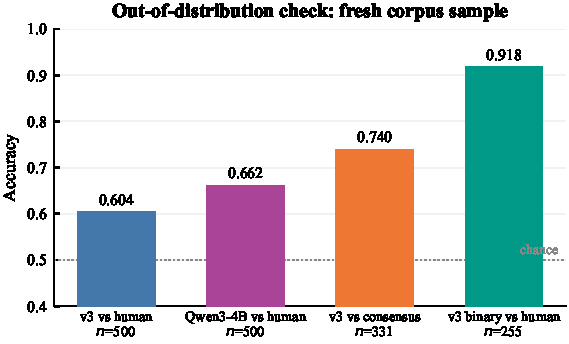
\includegraphics[width=0.8\textwidth]{fig_lab500.pdf}
\caption{lab500 按“评估者—参照”配对的准确率。二分类任务的
泛化远好于三分类。}
\label{fig:lab500}
\end{figure}

\paragraph{发现。}
\begin{enumerate}
  \item \textbf{差距真实存在但高度集中。} 三分类准确率降至
        60--74\%，而二分类（正面对负面，$n=255$）仍保持
        91.8\%——极性很容易，失败的是中性边界。
  \item \textbf{瓶颈是标注歧义而非模型容量。} 两个独立 LLM
        标注员之间的一致率仅 66.2\%；一个在 400 条域内标签上
        训练的 MacBERT 模型对留出标签的 OOF 复现率也只有
        60\%。语料中简短、缺乏上下文的评论（中位 25 字，对比
        金标 80 字）本质上是有歧义的——该数据上的有效上限
        远低于金标基准。
  \item \textbf{难度可预测。} 教师认为容易的样本（置信度
        $\ge 0.7$）上所有标注对都达到 0.757；难样本约
        0.53。这一差距是难度差异，而非训练泄漏的证据
        （金标重叠仅 3/600 行，可忽略）。
\end{enumerate}

我们将其作为局限性如实报告，而非掩盖的缺陷：这正是本项目投入
语料规模伪标注的原因，也指明了未来工作方向（对短评进行人工
标注）。

%=====================================================================
\section{局限性与效度威胁}
\label{sec:limits}

\begin{itemize}
  \item \textbf{领域狭窄。} 金标集是来自\emph{单一影片页面}的
        600 条评论；lab500 研究证实分布偏移是外部效度的主要威胁。
  \item \textbf{伪标签天花板。} 伪标签继承教师偏差；飞轮在一轮
        后饱和（第二轮平均置信度 0.986 = 记忆化）。
  \item \textbf{统计功效。} 在 $n=600$ 下，低于约 1pp 的差异
        无法分辨；语料规模的结论依赖评分相关性证据，而非人工标签。
  \item \textbf{lab500 标签为 LLM 辅助}，并非金标准人工标注；
        60--74\% 的区间应理解为“与现有标注者的一致程度”，其
        下界受 66\% 的 LLM—LLM 一致率本身约束。
  \item \textbf{工程约束。} ROCm/Windows GPU 栈在 13 亿参数特征
        提取期间需要驱动级重启；推理延迟数字为单卡测量值。
\end{itemize}

%=====================================================================
\section{结论与未来工作}
\label{sec:conclusion}

在真实的低资源中文情感任务上，语料规模伪标注是杠杆最高的成分：
它将中性召回率从 54\% 提升至 71\%，并使单一紧凑学生几乎追平
多模型集成。基于语料训练中性检测器的专家分解带来了进一步的
已验证增益。仅靠星级评分不足以构成监督——这是实测结论而非
假设。同样重要的是，我们诚实的分布外研究表明，金标基准高估了
短评论上的真实三分类表现；不过二分类极性泛化良好（91.8\%）。

未来工作：(i) 扩充对短评的人工标注至 1{,}000+ 行，以收窄置信
区间并厘清中性边界；(ii) 使用更强的 LLM 教师对语料重新标注，
注入学生缺乏的知识；(iii) 测试 MacBERT-large 学生与完整的
271K 不平衡池；(iv) 采用领域对抗或多领域训练以弥合金标$\to$
语料的差距。

%=====================================================================
\section*{可复现性}
\addcontentsline{toc}{section}{可复现性}

\begin{sloppypar}
全部脚本、交叉验证预测与实验记录位于项目仓库
（\url{https://github.com/shuakami/douban-sentiment}）。911K 语料为外部数据（研究用途，不再分发）；训练好的检查点发布于
\url{https://huggingface.co/Shuakami/douban-sentiment-weights}。
完整的 预处理$\to$伪标注$\to$训练$\to$评估 流水线均有脚本端到端
覆盖。关键产物：\code{out/ens\_lite\_3class\_v3.json}（部署的
三分类 OOF 预测与概率）、\code{out/lab500\_*}（分布外研究）、
\code{scripts/}（全部训练/评估代码）、\code{PAPER.md}（精简版
报告）。硬件：AMD RX 9070 GRE，ROCm，PyTorch bf16。
\end{sloppypar}

%=====================================================================
\appendix
\section{训练细节与可复现性}
\label{app:repro}

\subsection{超参数}

\begin{table}[H]
\centering\small
\caption{部署流水线的关键超参数。}
\label{tab:hparams}
\begin{tabular}{lll}
\toprule
组件 & 设置 & 取值 \\
\midrule
蒸馏学生   & 骨干 & \code{hfl/chinese-macbert-base} \\
           & 蒸馏 $\alpha/\tau$ & 0.5 / 2 \\
           & epoch 数 / 最大长度 & 8 / 256 \\
           & 折数（OOF） & 5 \\
判别器头   & 骨干 & MegatronBERT-1.3B（冻结） \\
           & 特征 & 4096 维（CLS + 均值池化） \\
           & 头部 & 2 层 MLP \\
中性检测器 & 骨干 & MacBERT-base \\
           & 训练行数 & 115{,}000（每类上限 6 万，2 epoch） \\
伪标签池   & 置信度 & $\max p \ge 0.7$ \\
           & 行数 & 271{,}905（56.5K/68.6K/146.8K） \\
校准       & 方法 & 温度缩放 \\
           & $T$ & 0.37（金标 NLL 拟合） \\
集成权重   & dep & 学生 1 : 判别器 2 \\
           & spec 混合 & 0.5 \\
           & $p_n$ 配比 & 0.6 判别器头 : 0.4 语料检测器 \\
\bottomrule
\end{tabular}
\end{table}

\subsection{产物清单}

\begin{itemize}
  \item \code{out/ens\_lite\_3class\_v3.json} —— 部署的三分类
        OOF 预测与概率（全部 600 行）。
  \item \code{out/ens\_lite\_binary.json} —— 部署的二分类 OOF。
  \item \code{out/lab500\_*} —— 分布外研究：样本、双 LLM 标签、
        预测、交叉验证结果。
  \item \code{scripts/} —— 端到端流水线，涵盖语料预处理、伪标注、
        语料头训练、蒸馏与集成评估（完整脚本列表见仓库）。
  \item \code{web/} + \code{web-ui/} —— FastAPI 后端与 React 演示。
\end{itemize}

\subsection{环境}

Python 3.12，PyTorch（ROCm），\code{transformers}，AMD RX 9070 GRE
GPU。所有 GPU 任务串行执行（并发任务会使 ROCm/Windows 栈崩溃）。
模型权重：每个 MacBERT 学生约 400MB；共享的 MegatronBERT-1.3B
骨干；部署总占用不足 4GB。冷启动约 14 秒，热态推理约 0.1 秒/条。

%=====================================================================
\begin{thebibliography}{99}\small

\bibitem[Devlin et al.(2019)]{devlin2019}
J.~Devlin, M.-W.~Chang, K.~Lee, K.~Toutanova.
\newblock \emph{BERT: Pre-training of Deep Bidirectional Transformers for Language Understanding}.
\newblock In \emph{Proceedings of NAACL-HLT}, pages 4171--4186, 2019.
\newblock \url{https://arxiv.org/abs/1810.04805}.

\bibitem[Liu et al.(2019)]{liu2019}
Y.~Liu, M.~Ott, N.~Goyal, J.~Du, M.~Joshi, D.~Chen, O.~Levy, M.~Lewis,
L.~Zettlemoyer, V.~Stoyanov.
\newblock \emph{RoBERTa: A Robustly Optimized BERT Pretraining Approach}.
\newblock \emph{arXiv preprint arXiv:1907.11692}, 2019.
\newblock \url{https://arxiv.org/abs/1907.11692}.

\bibitem[Cui et al.(2020)]{cui2020}
Y.~Cui, W.~Che, T.~Liu, B.~Qin, Z.~Yang, S.~Wang, G.~Hu.
\newblock \emph{Revisiting Pre-Trained Models for Chinese Natural Language Processing}.
\newblock In \emph{Findings of EMNLP}, pages 657--668, 2020.
\newblock \url{https://arxiv.org/abs/2004.13922}.

\bibitem[Wang et al.(2020)]{wang2020}
W.~Wang, B.~Bi, M.~Yan, C.~Wu, Z.~Bao, J.~Xia, L.~Peng, L.~Si.
\newblock \emph{StructBERT: Incorporating Language Structures into Pre-training for Deep Language Understanding}.
\newblock In \emph{International Conference on Learning Representations (ICLR)}, 2020.
\newblock \url{https://arxiv.org/abs/1908.04577}.

\bibitem[Sun et al.(2019)]{sun2019}
Y.~Sun, S.~Wang, Y.~Li, S.~Feng, X.~Chen, H.~Zhang, X.~Tian, D.~Zhu,
H.~Tian, H.~Wu.
\newblock \emph{ERNIE: Enhanced Representation through Knowledge Integration}.
\newblock \emph{arXiv preprint arXiv:1904.09223}, 2019.
\newblock \url{https://arxiv.org/abs/1904.09223}.

\bibitem[IDEA-CCNL(2023)]{idea2023}
IDEA-CCNL.
\newblock \emph{Erlangshen-MegatronBert-1.3B-Sentiment}: model card and weights.
\newblock Hugging Face model hub, 2023.
\newblock \url{https://huggingface.co/IDEA-CCNL/Erlangshen-MegatronBert-1.3B-Sentiment}.

\bibitem[Kim(2014)]{kim2014}
Y.~Kim.
\newblock \emph{Convolutional Neural Networks for Sentence Classification}.
\newblock In \emph{Proceedings of EMNLP}, pages 1746--1751, 2014.
\newblock \url{https://aclanthology.org/D14-1181/}.

\bibitem[Socher et al.(2013)]{socher2013}
R.~Socher, A.~Perelygin, J.~Wu, J.~Chuang, C.~D.~Manning, A.~Y.~Ng, C.~Potts.
\newblock \emph{Recursive Deep Models for Semantic Compositionality Over a Sentiment Treebank}.
\newblock In \emph{Proceedings of EMNLP}, pages 1631--1642, 2013.
\newblock \url{https://aclanthology.org/D13-1170/}.

\bibitem[Pang and Lee(2008)]{pang2008}
B.~Pang, L.~Lee.
\newblock \emph{Opinion Mining and Sentiment Analysis}.
\newblock \emph{Foundations and Trends in Information Retrieval}, 2(1--2):1--135, 2008.
\newblock \url{https://doi.org/10.1561/1500000011}.

\bibitem[Tan and Zhang(2008)]{tan2008}
S.~Tan, J.~Zhang.
\newblock \emph{An Empirical Study of Sentiment Analysis for Chinese Documents}.
\newblock \emph{Expert Systems with Applications}, 34(4):2622--2629, 2008.
\newblock \url{https://doi.org/10.1016/j.eswa.2007.05.028}.

\bibitem[Yarowsky(1995)]{yarowsky1995}
D.~Yarowsky.
\newblock \emph{Unsupervised Word Sense Disambiguation Rivaling Supervised Methods}.
\newblock In \emph{Proceedings of ACL}, pages 189--196, 1995.
\newblock \url{https://aclanthology.org/P95-1026/}.

\bibitem[Lee(2013)]{lee2013}
D.-H.~Lee.
\newblock \emph{Pseudo-Label: The Simple and Efficient Semi-Supervised Learning Method for Deep Neural Networks}.
\newblock ICML 2013 Workshop on Challenges in Representation Learning, 2013.

\bibitem[Arazo et al.(2020)]{arazo2020}
E.~Arazo, D.~Ortego, P.~Albert, N.~E.~O'Connor, K.~McGuinness.
\newblock \emph{Pseudo-Labeling and Confirmation Bias in Deep Semi-Supervised Learning}.
\newblock \emph{arXiv preprint arXiv:1908.02983}, 2020.
\newblock \url{https://arxiv.org/abs/1908.02983}.

\bibitem[Ratner et al.(2017)]{ratner2017}
A.~Ratner, S.~H.~Bach, H.~R.~Ehrenberg, J.~Fries, S.~Wu, C.~R\'e.
\newblock \emph{Snorkel: Rapid Training Data Creation with Weak Supervision}.
\newblock \emph{Proceedings of the VLDB Endowment}, 11(3):269--282, 2017.
\newblock \url{https://arxiv.org/abs/1711.10160}.

\bibitem[Xie et al.(2020)]{xie2020}
Q.~Xie, M.-T.~Luong, E.~Hovy, Q.~V.~Le.
\newblock \emph{Self-Training with Noisy Student Improves ImageNet Classification}.
\newblock In \emph{Proceedings of CVPR}, 2020.
\newblock \url{https://arxiv.org/abs/1911.04252}.

\bibitem[Sohn et al.(2020)]{sohn2020}
K.~Sohn, D.~Berthelot, N.~Carlini, Z.~Zhang, H.~Zhang, C.~A.~Raffel,
E.~D.~Cubuk, A.~Kurakin, C.-L.~Li.
\newblock \emph{FixMatch: Simplifying Semi-Supervised Learning with Consistency and Confidence}.
\newblock In \emph{Advances in NeurIPS}, 2020.
\newblock \url{https://arxiv.org/abs/2001.07685}.

\bibitem[Hinton et al.(2015)]{hinton2015}
G.~Hinton, O.~Vinyals, J.~Dean.
\newblock \emph{Distilling the Knowledge in a Neural Network}.
\newblock \emph{arXiv preprint arXiv:1503.02531}, 2015.
\newblock \url{https://arxiv.org/abs/1503.02531}.

\bibitem[Gou et al.(2021)]{gou2021}
J.~Gou, B.~Yu, S.~J.~Maybank, D.~Tao.
\newblock \emph{Knowledge Distillation: A Survey}.
\newblock \emph{International Journal of Computer Vision}, 129(6):1789--1819, 2021.
\newblock \url{https://arxiv.org/abs/2006.05525}.

\bibitem[Joulin et al.(2017)]{joulin2017}
A.~Joulin, E.~Grave, P.~Bojanowski, T.~Mikolov.
\newblock \emph{Bag of Tricks for Efficient Text Classification}.
\newblock In \emph{Proceedings of EACL}, pages 427--431, 2017.
\newblock \url{https://aclanthology.org/E17-2068/}.

\bibitem[Reimers and Gurevych(2019)]{reimers2019}
N.~Reimers, I.~Gurevych.
\newblock \emph{Sentence-BERT: Sentence Embeddings using Siamese BERT-Networks}.
\newblock In \emph{Proceedings of EMNLP-IJCNLP}, pages 3982--3992, 2019.
\newblock \url{https://arxiv.org/abs/1908.10084}.

\bibitem[Guo et al.(2017)]{guo2017}
C.~Guo, G.~Pleiss, Y.~Sun, K.~Q.~Weinberger.
\newblock \emph{On Calibration of Modern Neural Networks}.
\newblock In \emph{Proceedings of ICML}, pages 1321--1330, 2017.
\newblock \url{https://proceedings.mlr.press/v70/guo17a.html}.

\bibitem[Qwen Team(2025)]{qwen2025}
Qwen Team.
\newblock \emph{Qwen3: Technical Report and Model Release}.
\newblock GitHub repository and model documentation, 2025.
\newblock \url{https://github.com/QwenLM/Qwen3}.

\bibitem[Gilardi et al.(2023)]{gilardi2023}
F.~Gilardi, M.~Alizadeh, M.~Kubli.
\newblock \emph{ChatGPT Outperforms Crowd-Workers for Text-Annotation Tasks}.
\newblock \emph{Proceedings of the National Academy of Sciences}, 120(30):e2305016120, 2023.
\newblock \url{https://doi.org/10.1073/pnas.2305016120}.

\bibitem[T\"ornberg(2023)]{tornberg2023}
P.~T\"ornberg.
\newblock \emph{ChatGPT-4 Outperforms Experts and Crowd Workers in Annotating
Political Twitter Messages with Zero-Shot Learning}.
\newblock \emph{arXiv preprint arXiv:2304.06588}, 2023.
\newblock \url{https://arxiv.org/abs/2304.06588}.

\bibitem[Dietterich(1998)]{dietterich1998}
T.~G.~Dietterich.
\newblock \emph{Approximate Statistical Tests for Comparing Supervised Classification Learning Algorithms}.
\newblock \emph{Neural Computation}, 10(7):1895--1923, 1998.
\newblock \url{https://doi.org/10.1162/089976698300017197}.

\bibitem[Dem\v{s}ar(2006)]{demsar2006}
J.~Dem\v{s}ar.
\newblock \emph{Statistical Comparisons of Classifiers over Multiple Data Sets}.
\newblock \emph{Journal of Machine Learning Research}, 7:1--30, 2006.
\newblock \url{https://jmlr.org/papers/v7/demsar06a.html}.

\bibitem[Efron and Tibshirani(1993)]{efron1993}
B.~Efron, R.~J.~Tibshirani.
\newblock \emph{An Introduction to the Bootstrap}.
\newblock Chapman \& Hall, London, 1993.

\bibitem[McNemar(1947)]{mcnemar1947}
Q.~McNemar.
\newblock \emph{Note on the Sampling Error of the Difference Between Correlated Proportions or Percentages}.
\newblock \emph{Psychometrika}, 12(2):153--157, 1947.
\newblock \url{https://doi.org/10.1007/BF02295996}.

\bibitem[csuldw(2019)]{douban2024}
csuldw. Moviedata-10M: a large-scale Douban movie dataset (140{,}502
films, 4{,}428{,}475 comments, collected 2019).
\newblock AntSpider project, Central South University, 2019.
\newblock \url{https://github.com/csuldw/AntSpider}. Research use only;
the raw corpus is not redistributed here.

\end{thebibliography}

\end{document}
